% !TEX root = ../thesis_main.tex
%
%
%
%%%% --- * --- %%%%	
\chapter{Background}
\label{intro_chapter}
\label{nuclear_chapter}
Within nature, there exist four fundamental forces governing the interactions of particles with one another:  electromagnetism, the nuclear weak force, the nuclear strong force, and gravity.  This work seeks to probe the nature of the weak nuclear force on its most fundamental level through observations of beta decay, a process which results directly from the action of the weak nuclear force.  Through kinematic observations of the decay products, much can be learned about the form of the weak nuclear force's coupling, through which beta decay proceeds.  Prior experiments have shown that this coupling is dominated by a combination of operators that behave as vectors and axial-vectors under Lorentz transformation, however 
%vector and axial-vector operators, but 
the possibility of a non-dominant contribution from other types of operators, such as scalars and tensors, cannot be ruled out entirely.  This is the domain of precision measurements.  

\section{Introduction}
\label{section:intro}
Within our present understanding of physics, there are four fundamental forces governing the interactions of particles with one another:  electromagnetism, the nuclear weak force, the nuclear strong force, and gravity.  These forces are considered to be distinct from one another by virtue of their differing behaviours, however attempting to unify them within a single theoretical framework has been a major focus of later 20th- and early 21st century physics to date.  The effort has been met with only partial success, and the resulting theoretical framework is collectively known as the \ac{SM}.

The standard model provides a quantum mechanical description for
the behaviour of three of the four fundamental forces:  electromagnetism, the nuclear weak force, and the nuclear strong force.  The \ac{SM} notably does not describe gravitational processes --- despite extensive efforts, the gravitational force has thus far defied all attempts to describe it in a fully quantum mechanical way, though this remains an active field of research.  

%
Each force has its own specific mediating particle(s) which couple only to a particular type of (generalized) charge, and therefore interact only with particles that possess that charge.  For example, the gravitational charge is \emph{mass}, and (at least within a simplified particle physics model) gravity acts only on objects that possess mass.~\aside{Can I turn this into a footnote?  It's not true because the curvature of spacetime also affects photon trajectories, and there even exist (unstable) (quasi-?) bound states comprised *only* of photons, as in e.g. Aichelburg-Sexl.}  With only a single type of charge and no negative masses, the gravitational force can only ever be attractive.
%
By constrast, the electromagnetic force couples to both positive and negative electric charges, and can produce both attractive and repulsive forces.  Both the electromagnetic and gravitational forces are mediated by massless force-carrying particles (the photon and still-theoretical graviton, respectively), a property which implies that the amount of flux per unit solid angle is constant over all distance scales, and Gauss's Law holds true.

\begin{figure}[h!t!b!]
	\centering
	\includegraphics[width=.75\linewidth]{Figures/feynmandiagrams_general_placeholdercropped.pdf}
	\note[tag]{Fix Feynman diagram vertex placeholder figure.}
	\caption[An exhaustive list of weak vertices]{An exhaustive list of weak vertices.  All possible Feynman diagram vertices involving $W^+$, $W^-$, or $Z^0$ bosons are shown, and the usual rules apply.  These vertices show the types of interactions that can occur between the bosons mediating the weak force, and other types of particles.  Only the fundamental vertices are shown, meaning that these diagrams are in some sense incomplete.  At the energy scales available in everyday life, the $W$ and $Z$ bosons act only as an intermediary between two such vertices.}	
	\label{fig:feynmandiagrams_general}
\end{figure}

In the case of the nuclear weak force, which will be the primary concern within this thesis, 
the notion of generalized charge is no longer entirely straightforward to apply.
We must rely instead on a list of allowed Feynman diagram vertices to describe the types of interaction that are possible (see Fig.~\ref{fig:feynmandiagrams_general}).  We note that the weak force involves three mediating particles --- $W^+$, $W^-$, and $Z^0$ bosons --- and these mediators can interact with both (anti-)quarks and (anti-)leptons.  The $W^+$ and $W^-$ particles also carry electric charge, which must be separately conserved in any interaction,~\aside{(wait, is that true?  what about with the photon vertex? ....I think it's fine.....} but the $Z^0$ is electrically neutral.  All three are massive, which implies that the strength of the weak force falls off more rapidly as distance increases, and Gauss's Law does not apply. 


With a comparatively large number of possible vertex types, it can be challenging to develop an intuition about the behaviour of the weak force. 
Perhaps the most well known physical behaviour that arises from the nuclear weak force is beta decay. 
Indeed, beta decay
offers one of the most readily accessible experimental windows to the workings of the nuclear weak force.

Although it is now generally well understood, beta decay still presents a unique opportunity for precision measurements to search for exotic physics beyond the Standard Model within the weak coupling.
By observing the kinematics and angular correlations involved in the decay process, one gains access to a wealth of information about the 
laws underpinning the decay process, and the weak force as a whole.  



%%%% --- * --- %%%%	
\section{A Historical Look at Beta Decay and the Weak Interaction}

We consider the historical development of our scientific understanding of beta decay and the nuclear weak force.  This is a historically rich topic, and a full discussion is beyond the scope of this document, however we shall attempt to touch on some highlights.

Radioactivity was first observed in 1896 by Henri Becquerel in uranium, and this landmark discovery set off a flurry of activity in the field~\cite{becquerel1896}.
Ernest Rutherford noted in 1899 that the particles emitted by a sample of uranium could be classified into two groups based on how readily they were absorbed in materials -- alpha particles are easily absorbed, while beta particles are more penetrating~\cite{rutherford1899}.  A third and even more penetrating type of radioactive emission was observed in 1900 by Paul Villard, who made no attempt to give it a name -- but within a few years, Rutherford's naming convention had been applied and this third type of particle became known as a gamma ray~\cite{villard1900}\cite{rutherford1903}.  

\note{Rutherford discovered that:  half-life.  [76]=E. Rutherford, \emph{Phil. Mag.} \textbf{49}, 1, 1900.  Thorium.  Rn220.  ...but also, *I* got this from Abraham Pais.}

When, in 1900, Becquerel measured the charge-to-mass ratio of emitted beta ($\beta^-$) radiation and found that it was the same as that of the electron, he proposed that these must be the same particle~\cite{becquerel1900},~\aside{I think.  Also, I think that's the right citation..} and in 1903~\aside{or possibly 1901?} Rutherford and Soddy demonstrated that the processes of alpha and beta decay both transmute the original chemical element into another\cite{rutherfordsoddy1903}.


Despite these early successes, in 1911 Lise Meitner and Otto Hahn noticed that beta particles are emitted with a variety of different kinetic energies,~\aside[tag]{citation needed} and in 1914 James Chadwick
%%~\aside{citation needed.  also, maybe it was a bunch of people, 1914-1927.  
%%\\
%%Chadwick's original:  Chadwick, J. (1914). "Intensitätsverteilung im magnetischen Spektren der β-Strahlen von Radium B + C". Verhandlungen der Deutschen Physikalischen Gesellschaft (in German). 16: 383–391.  
%%\\
%%Maybe also Charles Drummond Ellis?  
%%\\
%%Ellis and Wooster:  Ellis, C. D.; Wooster, W. A. (1927). "The Continuous Spectrum of β-Rays". Nature. 119 (2998): 563–564. doi:10.1038/119563c0. S2CID 4097830.  } 
demonstrated that energies of emitted beta particles formed a continuous distribution.  The physics community was baffled for years by the fact that it seemed impossible to predict the energy of a beta particle emitted by a particular process;  if the emitted beta simply took on the difference in energy between the initial and final states, then surely that energy should be a fixed, unchanging value for a paricular transition. 

%should be a fixed amount of energy for a given transition.  
Finally, in 1930, a frustrated Wolfgang Pauli famously proposed that if an additional small, neutral, difficult to detect particle were emitted simultaneously with the beta and allowed to carry away a varying amount of energy, then this accounting trick could account for the continuous beta energy spectrum.
%could account for the continuous beta energy spectrum, by carrying away whatever fraction of the
%This new particle was dubbed a ``neutron'' 
He named this particle a ``neutron'' -- though today we refer to that same particle as a(n) ``(anti-)neutrino,'' and use the name ``neutron'' for an entirely different particle\cite{PauliNeutrino1978}.  \aside{Fermi renamed it, because Italian.}

%When Enrico Fermi offered a quantitative description of 
Pauli's 1930 insight paved the way for Enrico Fermi to propose a quantitative description of the nuclear weak force and the beta decay processes resulting from it.  He modeled the weak force as a contact interaction with zero range --- a very good approximation.  After being rejected by \emph{Nature} in 1933, Fermi's seminal theory of beta decay was published in both Italian and German journals the following year \cite{AbrahamPais} \cite{Fermi1934Italian} \cite{Fermi1934German}.
%\aside[done]{Citation is:  Pais, Abraham (1986). Inward Bound. Oxford: Oxford University Press. p. 418. ISBN 0-19-851997-4. \cite{AbrahamPais} }  
Because of its powerful predictive ability together with its generalized quantum mechanical approach, Fermi's model forms the basis upon which modern beta decay calculations have been built.  With one of its major results, now commonly known as Fermi's Golden Rule, still routinely used, the introduction of Fermi's model arguably marks the beginning of our modern understanding of beta decay.

The mid 1930s was a busy time 
%1934 was a busy year 
for our understanding of beta decay.  In addition to the publication of Fermi's model in 1934, this year also marks the first discovery of $\beta^+$ radiation, for which Irène and Frédéric Joliot-Curie later received a Nobel prize, and the proposal by Gian-Carlo Wick of the electron capture mechanism for beta decay.  
The electron capture theory was fleshed out further in 1935-1936 by Yukawa and Sakata\aside{and others?},\aside{Yukawa and Sakata first names?} and first observed in 1937 by Luis Alvarez.  Meanwhile, in 1936 George Gamow and Edward Teller improved upon Fermi's model by including a mechanism to potentially change the nuclear spin\cite{GamowTeller}, and to this day, beta decay transitions are still routinely classified as following Fermi or Gamow-Teller (or mixed) selection rules.

%~\aside{omg, I can't just give first names for only the non-Asian people...}
%\note[tag]{Gamow-Teller in 1936\cite{GamowTeller}. }
%1934 was also the year when Wick proposed the electron capture mechanism for beta decay, later observed by Luis Alvarez in 1937.  \aside{Yukawa and others totes helped flesh out the theory behind E.C.  Or possibly they proposed it first?  who even knows.}
Over the next few years, developments within the field of nuclear physics were largely directed elsewhere, but beta decay returned to scientific prominence with T. D. Lee and C. N. Yang's 1956 suggestion~\aside[tag]{Probably point out that this thing is the basis for the model of the weird-ass currents I'm looking for.  They made a (nucleon-level) Hamiltonian with *everything*.} 
that, contrary to the community's prior expectation, parity may not be conserved within beta decay processes\cite{LeeYang}.
~\aside{their hamiltonian operates at the nucleon level, because they hadn't discovered quarks yet.  also, this is the basis for where we're going with this experiment.  shows all possible Lorentz-invariant contributions to the thingy. V,A,S,T,P.  I don't think they knew about W and Z bosons either.}  The proposition was rapidly put to the test by C.S. Wu's landmark 1957 measurement of $^{60}$Co, confirming that beta decay violates parity conservation and simultaneously paving the way for the Nobel prize to be awarded to Lee and Yang that same year~\cite{wu}.~\aside{nobel prize citation?}
~\aside{For a while everyone thought it was S,T.  But it turns out it's V,A.  Ben cites these guys for S,T:  \cite{RustadRuby1955tensor}\cite{BurgyEpstein1957scalartensor}.  though, the one article is before Wu. Also, I can't access these things.  Look at JTW's refs maybe..}
%\note{... a discovery which earned Lee and Yang a Nobel prize.  Wu's discovery earned Lee and Yang the 1957 Nobel Prize.}

Subsequent experiments demonstrated that not only was parity non-conserved in a beta decay transition, it is (as near as we can collectively tell) \emph{maximally} violated.  \aside{cite someone for maximal parity violation.}
Though early experiments suggested that the couplings were likely comprised of 
%so-called 
scalar and tensor interactions,\aside{cite someone for S,T !  John suggests 6He $\abetanu$ for the tensor.} Feynman and Gell-Mann first postulated the correct $(V-A)$ form of the interaction in 1958 by invoking an analogy with the photon, and this was eventually borne out by experimental evidence\cite{FeynmanGellMann1958}.  (See Sec.~\ref{sec:SMandBeyond} for further discussion on the form of weak interaction couplings.)
\aside{cite someone for $(V-A)$ evidence}

In the following years, the theory behind the nuclear weak force was developed further, and eventually merged with the theory of electromagnetism as the electroweak force.  The framework for \ac{QED} had already been largely developed between 1946 and 1950 by Shinichiro Tomonaga, Julian Schwinger, Richard Feynman, and others.  The theory was fully covariant, meaning that it behaves properly under a Lorentz transformation.  The work of Schwinger, and independently, Tomonaga, developed much of the methodology behind renormalization, which is now considered to be a mathematical necessity in any modern quantum field theory\cite{tomonaga1946}\cite{schwinger1948covariant}\cite{feynman1949spacetime}\cite{feynman1949positrons}\cite{feynman1950}\cite{dyson1949theories}.  ~\aside{QED as a "template" for other theories.}


\note{From Wikipedia:  ``In 1957, Robert Marshak and George Sudarshan and, somewhat later, Richard Feynman and Murray Gell-Mann proposed a $V-A$ Lagrangian for weak interactions.''
\\...\\
``In the Standard Model, the $W^\pm$ and $Z^0$ bosons, and the photon, are produced through the spontaneous symmetry breaking of the electroweak symmetry SU(2) × U(1)Y to U(1)em, ...''
}

Following the success of QED, there was a push from the physics community to create a similar theory to model the nuclear weak force.  
%
Lee and Yang, and Feynman and Gell-Mann, produced two notable early examples of a weak force Lagrangian written, like the theory of electromagnetism, in terms of Lorentz-transforming currents\cite{LeeYang}\cite{FeynmanGellMann1958}.  Yang and Mills took a more mathematical approach, and their 1954 non-abelian gauge theory \cite{YangMills1954} lies at the foundation of electroweak unification.  
%

In 1961, Sheldon Glashow extended some of Schwinger's work to model the nuclear weak force,  adding an explicit mass term (i.e., to make the force mediating particles massive).  The model included the $W^+$ and $W^-$ bosons needed to explain beta decay, and for the first time, a neutral $Z^0$ boson.  With the explicit mass term, the theory was not renormalizable, and since there had been no experimental hint of the $Z^0$, Glashow himself discounted the model, and it initially received little attention.  In 1964, Abdus Salam and John Clive Ward proposed a similar theory, this time including the photon as well as $W^\pm$ and $Z^0$ bosons -- however they, too, relied on explicit symmetry breaking to provide a mass for the $W^\pm$ and $Z^0$ bosons\cite{Glashow1959}\cite{Glashow1961}\cite{SalamWard1964}.


With the development of the Higgs mechanism in 1964, which provided an indirect mechanism for gauge bosons to gain a non-zero mass spontaneously without the need to explicitly add a mass term\cite{Higgs1964EnglertBrout}\cite{Higgs1964Higgs}\cite{Higgs1964GuralnikHagenKibble}\cite{BroutEnglertArXiv}\cite{guralnik2009}, it was perhaps only a matter of time before Salam and, separately, Steven Weinberg applied that mechanism to the weak force in 1967, producing a theory of electroweak interaction that was potentially renormalizable\cite{Weinberg1967}\cite{salam1968}.~\aside{...and then Weinberg immediately went and predicted the masses of W and Z bosons.  Did he do a good job??}  It was not until 1971 that Gerardus 't Hooft and Martinus Veltman proved that this class of theories actually \emph{is} renormalizable, thereby making the Weinberg-Salam model of the electroweak force a much more viable theory\cite{thooftveltman1972}.

The Weinberg-Salam model of electroweak interactions was borne out by the experimental observation of the weak neutral current (i.e., the interaction mediated by the $Z^0$ boson) in 1973 at CERN's Gargamelle bubble chamber experiment\cite{gargamelle}.  The $W^\pm$ and $Z^0$ bosons themselves were first unambiguously observed at CERN's Super Proton Synchrotron in 1983\cite{UA1W}\cite{UA2W}\cite{UA1Z}\cite{UA2Z} -- with the $W^\pm$ and $Z^0$ being quite massive in comparison to other fundamental particles, earlier experimental designs had not been powerful enough to reach the necessary energy scale.   \aside{Give the masses?  Maybe.}

Following the development of electroweak unification, 
%the complete Weinberg-Salam theory of electroweak interactions, 
theorists turned their attention to the nuclear strong force, which had been challenging to model in a mathematically rigorous way due to its property of growing \emph{stronger}, rather than weaker, at long distances.  The breakthrough came in 1973, when David Gross and Frank Wilczek, and separately, David Politzer developed a model of asymptotic freedom applied to the nuclear strong force\cite{gross1973asymptotically}\cite{gross1973ultraviolet}\cite{politzer1973reliable}.  

The completed theories of electroweak and strong interactions, together, formed the core of what has come to be known as the standard model of particle physics (\acs{SM}).  It is unclear exactly when this terminology developed, or who originated it, but it had certianly come into use by the mid-1970s, and the usage still persists\cite{PaisTreiman1975}\cite{weinberginterview2018}.  Notably, the only one of the fundamental forces not included under the umbrella of the standard model is the force of gravity, which is not compatible, as it is currently understood, with the quantum mechanical underpinnings of the standard model.  In the decades since, this incompatibility has been a major focus of inquiry for theoretical physicists, but the problem remains unresolved. 

\note[done]{Schwinger does renormalization, which makes QED go. Glashow~\cite{Glashow1959} extends it to the Z boson.  But now it's not renormalizable.  Salam and Ward~\cite{SalamWard1964} did a similar thing, but independently.   Then Weinberg (1967) did it but didn't know what to do with Z bosons~\cite{Weinberg1967}.  Until later.  Or something.  Then, 't Hooft (1971) proved that this thing was normalizable even with massive gauge bosons~\cite{thooft1971}.  Or at least, that's how Wikipedia describes it.  Also, in the end, electroweak unification was based on Yang-Mills (1954)~\cite{YangMills1954}, but their theory didn't really get that much attention initially because it was just a lot of boring math, and they couldn't figure out how to something something symmetry breaking.}

\note{Halliday doesn't remember Meitner+Hahn, and says Pauli's thing is 1927, but doesn't give a reference for it.
\\...\\
Also from Halliday:  Yukawa and Sakata first proposed the possibility of (orbital) electron capture in 1935-1936.  (What about Wick in 1934?)
\\...\\
Also-also:  Fermi in 1934 drew an analogy between emission of electrons and neutrinos from nuclei and emission of photons from excited atomic states.... (probably this gets us one step closer to isospin?)
}
\note{I could totes add a reference to Halliday's 1955 textbook (v2).}
%%\note{Other references to add include that one letter to the collaboration giving values of *things* from Ian Towner, 2011.}
\note{How do I reference a grant proposal?}
\note{separate ref. for the PRL's supp. mat.}

\note{alpha and beta decay:
\\
Rutherford, Ernest (1899). “Uranium radiation and the electrical conduction produced by it,” Philosophical Magazine 47, 109-163.
\\...\\
half-life:
\\
Rutherford, Ernest (1900). “A radio-active substance emitted from thorium compounds,” Philosophical Magazine 49, 1-14.
Or, possibly:
\\
Rutherford, Ernest (1906). Radioactive Transformations. London: Constable \& Co.
\\...\\
Transmutations?:
1902, 1903 --- rutherford and soddy.
}

\note{Here's some random thing John did in 2014:  \cite{somerandomthingJohndid2014}.  
\\
Here's some random thing that apparently all of TRINAT did in 2014:  \cite{somerandomthingTRINATdid2014}. 
\\
Here's Rob Pitcairn's thing:  \cite{Pitcairn2009}.  }
\note{I should probably cite Dan's thesis.  And Alexandre's too.\cite{alexandrethesis2008}.  Actually Dan's is already cited somewhere else, but here it is anyway:  \cite{dan_thesis}.  }

\note{$^8$Li limits on tensor currents from 2015, by Sternberg:  \cite{TensorLimits8Li2015}. 
\\...\\
Here's a thing I should probably cite, on the kinematic sensitivity of bFierz, from Gonzalez-Alonso and Naviliat-Cuncic:  \cite{KinematicFierz2016}.  }


\note[jbn, nolist]{
I think you've neglected where the fT value and prediction for Abeta come from, entirely, and still don't have an equation for b\_Fierz in terms of Cs and Ct.
\\...\\
You had a note to do this, and in desperation I encouraged you to leave it out.
I was wrong and Georg is right-- the whole SM prediction for Abeta makes no sense this way, and something about it needs to be there.
}
\note[jbn, nolist]{
there are two ways to add a dedicated section in ch 1:
\begin{itemize}
	\item i) by writing the equation for the rate in terms of Vud and rho (the G-T matrix element over Fermi squared), and saying Shidling et al. gets rho from that by assuming Vud from the 0+ to 0+ decays. (You had a note "Do the master equation!" which I think I said you needed to leave out, but I was probably wrong.) But then you have to define all the small corrections, which is a lot of physics.
	\item ii) Write the SM equation for Abeta in terms of rho, to give you the SM prediction for Abeta. State that recoil order corrections are in Appendix X. (If that's now a collaboration note? cite that there are recoil corrections considered in Appendix X-1 and a collaboration note).
	\item iii) Such a section would then naturally end with b\_Fierz in terms of Cs and Ct, a natural followup to what you've written.
	\\
"JTW does the Dirac matrix traces necessary to write down the decay rates in term of the Lee-Yang Lagrangian's parameters.
The prediction for b\_Fierz is " " which is zero in the SM." \textbf{even with recoil-order corrections} (there is no recoil order correction with the same m/Ebeta dependence).
\\
Then and only then will the final addition of the bFierz plot will make sense.
\end{itemize}
%
OR, more likely:
\\
\textbf{leave out i)}.
\\
Say in text that Shidling et al. (I've added the reference in a sticky note for the figure) hands you rho (the $M_{GT}/M_F$ ratio prediction) using as input the absolute rate, Vud from the 0+ to 0+ beta decays, and calculations of isospin mixing and radiative corrections (cite[shidling]) for details beyond the scope of this thesis. The sign of rho comes both from a shell model by Ian and by if it were flipped Abeta would be off by an enormous factor. 
\\...\\
Then you would just need \textbf{ii and iii}.
}


%%%% --- * --- %%%%	
\section{Beta Decay within the Standard Model and \; \mbox{Beyond}}
\label{sec:SMandBeyond}
In the most general sense, the process of beta decay is one in which a nucleon (proton or neutron) is transformed into a different nucleon (i.e., a neutron or proton, respectively) and a beta particle (a positron or electron, respectively) and neutrino are emitted.

At the nucleon level, there are three basic classes of beta decay processes:
\bea
	  n \;\;\rightarrow& p + e^- + \bar{\nu}_e        
\;\;\;\; \;\;\;\; \;\;\;\; \;\;\;\; 
	  & \beta^- \;\, \mathrm{Decay}    
\label{eq:betaminus_decay}  \\
	  p \;\;\rightarrow& n + e^+ + \nu_e              
\;\;\;\; \;\;\;\; \;\;\;\; \;\;\;\; 
	  & \beta^+ \;\, \mathrm{Decay}    
\label{eq:betaplus_decay}   \\
p + e^- \;\;\rightarrow& n + \nu_e, \;\;\;\; \;\;\;\; 
\;\;\;\; \;\;\;\; \;\;\;\; \;\;\;\; 
	   & \mathrm{Electron \;\, Capture}    
\label{eq:electroncapture}
\eea
where $p$ represents a proton and $n$ a neutron, $e^-$/$e^+$ represents an electron/positron (often referred to as a $\beta^-$/$\beta^+$), and $\nu_e$/$\bar{\nu}_e$ represents an electron neutrino/electron anti-neutrino.  In practice, these are often all simply referred to as "neutrinos".  

Of course, the processes of $\beta^+$ decay and electron capture are energetically disallowed for a proton not bound within a nucleus, but a free neutron will eventually undergo $\beta^-$ decay.  
%The rules for which of the above are energetically possible within a nucleus
Within the nucleus, rules of which processes are and are not energetically allowed are dependent on the specific nucleus in question.  Figure~\ref{fig:feynmandiagrams_betadecay} shows the Feynman diagrams associated with each of these processes.   
\begin{figure}[h!t!b!]
	\centering
	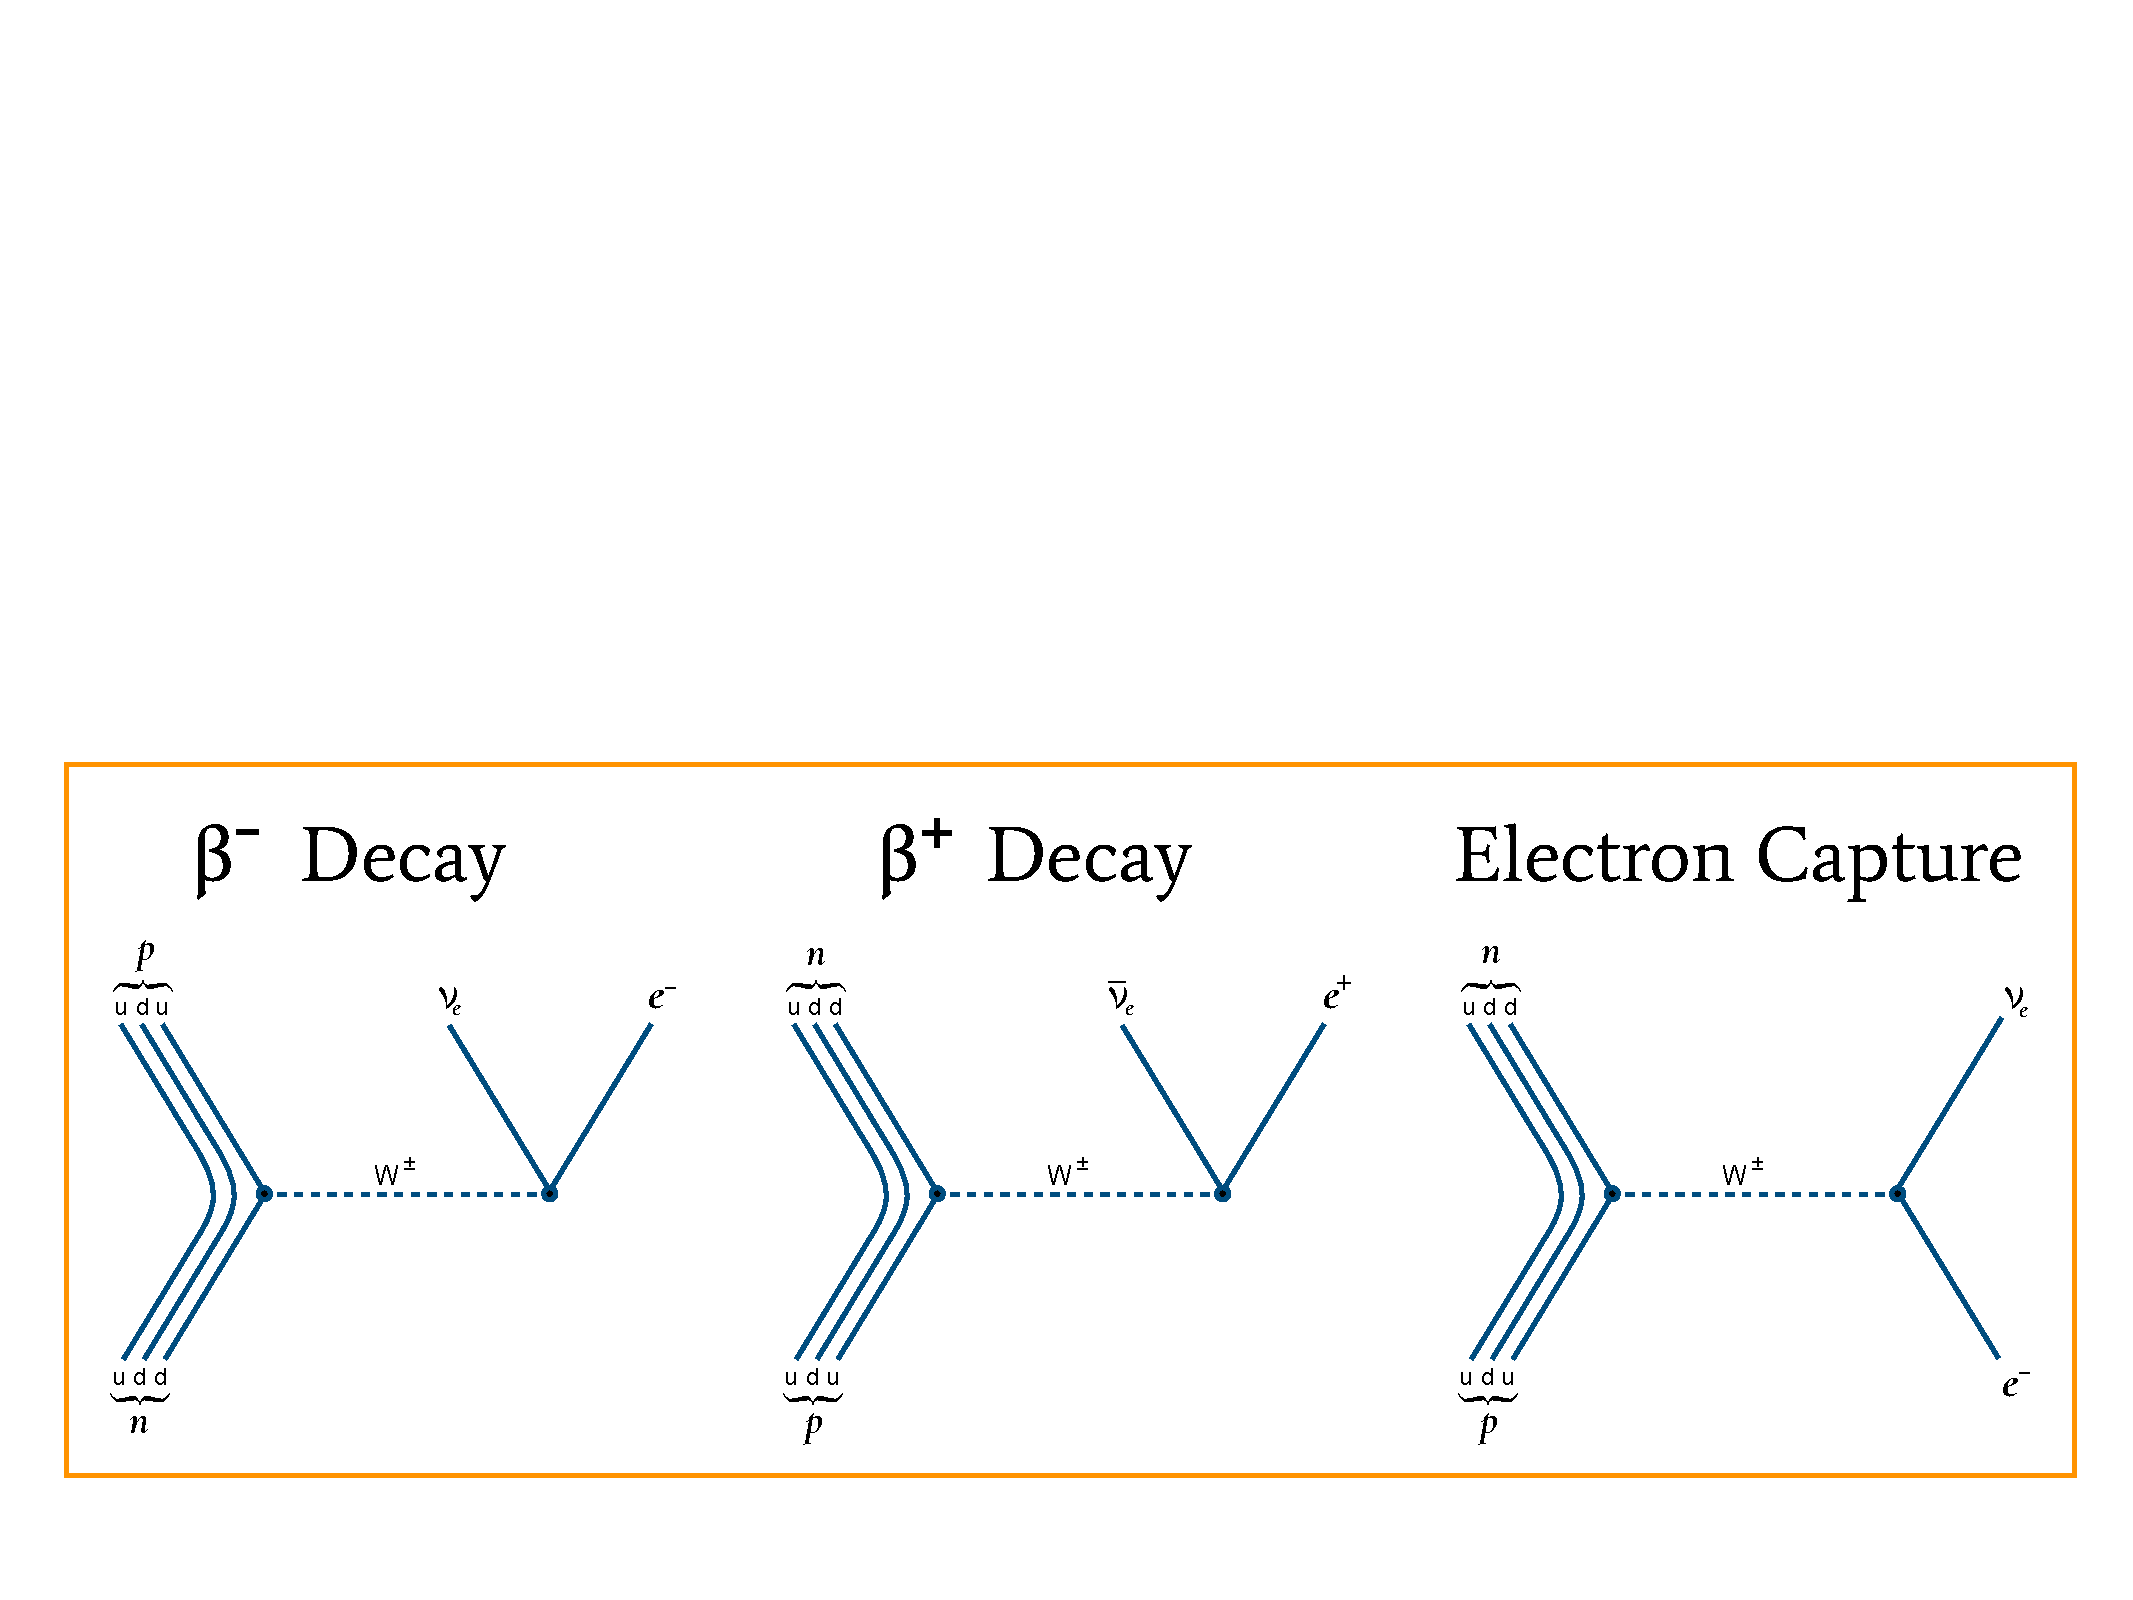
\includegraphics[width=1.0\linewidth]{Figures/BetaDecayFeynmanDiagrams.pdf}
%	\note[tag]{Fix beta decay Feynman diagram placeholder figure.}
	\caption[Beta Decay Feynman Diagrams]{Beta decay Feynman diagrams are drawn here to describe the three most common types of beta decay.  The interactions are mediated by massive $W^\pm$ bosons, resulting in an extremely limited range for the weak force.
%	 which have only a short range.
%		shown here at the nucleon(? sort of) level.    
	}	
	\label{fig:feynmandiagrams_betadecay}
\end{figure}

Energetic considerations aside, it is worthwhile to consider whether there might be any rules relating to the \emph{spin} of the nucleons before and after a decay, or the spins and angular correlations of the leptons that emerge.  Does the nucleon's spin flip during the decay process, or remain unchanged?  Are the decay products emitted preferentially in any particular direction?  Which direction are the beta and neutrino spins pointed in after they are emitted?  Angular momentum must, of course, be conserved -- but the question is \emph{how} it is to be conserved.  This question is not only at the heart of many modern precision measurements in beta decay physics, it has also been a driving force behind the development of much of our understanding of the nuclear weak force.

We must develop the tools with which these questions can be discussed.  We will begin by using Fermi's classic description of a beta decay as a transition that occurs with zero range:
\bea
\mathcal{M}_{fi} &=& G_F \int \bar{\psi}_f \, \mathcal{\hat{O}} \, \psi_i \,\textrm{d}V,
\label{eq:fermitransition}
\eea 
where $\mathcal{M}_{fi}$ is the transition matrix element between the final ($\psi_f$) and initial ($\psi_i$) states, and $G_F$ gives a measure of the strength of the coupling between states.  The integral is evaluated over phase space volume, and the operator $\mathcal{\hat{O}}$, which has yet to be determined, allows for a mathematical description of how the initial and final states must be related in order for a transition to occur.

Of course, this description represents a model of nuclear transitions which is highly simplified;  by neglecting the $W$ bosons that mediate the process and that we now know to be present, the result is a description of an interaction with zero range -- i.e., the leptons must be emitted from the exact place where the nucleon was transmuted.  Because the mediating $W$ bosons are so heavy ($m_W = 80.379(12)$\,GeV/$c^2$ ~\cite{pdg2018}), the range of the interaction is extremely limited, so the above turns out to be a very good description.  

This immediately gives rise to a rate law commonly known as Fermi's Golden Rule, 
\beq
\Gamma \;\; = \;\; \frac{1}{\tau}  \;\; = \;\; \frac{2\pi}{\hbar} \left| \mathcal{M}_{fi} \right|^2 \, \rho(E_f),
\eeq
which describes the relationship between the total transition rate $\Gamma$ (or equivalently the lifetime $\tau$), the transition matrix element $\mathcal{M}_{fi}$, and the available density of states at the final energy, $\rho(E_f)$.  We can also use this to write down the differential decay rate, 
\bea
\frac{\textrm{d}^5 \Gamma}{ \textrm{d} \Ebeta \textrm{d}\Omegahatbeta \textrm{d} \Omegahatnu } 
&=& \frac{1}{(2\pi)^5} \, \pbeta \Ebeta (E_0 - \Ebeta)^2 F_{\pm}(\Ebeta, Z^\prime) \left| \mathcal{M}_{fi} \right|^2,
\label{eq:fermidifferentialdecayrate}
\eea
where \aside{pretty sure I lost an $\hbar$.  Maybe no one will notice.  }
$\Ebeta$ and $\pbeta$ are the outgoing $\beta$'s (total) energy and momentum,
$E_0$ is the maximum possible $\beta$ energy associated with the transition, 
and $\FFpm$ is called a Fermi function (with $Z^\prime$ the proton number of the daughter), and is used to account for the electric force between the nucleus and the (charged) outgoing electron (top) or positron (bottom) \cite{Fermi1934Italian}\cite{Fermi1934German}\cite{krane}.  

With this description, the problem of characterizing the transition is reduced to determining the form of $\mathcal{\hat{O}}$.  %, or equivalently, $\mathcal{H}_{\mathrm{int}}$.  
Table~\ref{table:dirac_matrix_operators} provides a comprehensive list of all operators for which Lorentz invariance holds.  The complete transition operator $\mathcal{\hat{O}}$ must be comprised of a linear combination of these terms.  
% !TEX root = ../thesis_main.tex
%
%
%
%%%% --- * --- %%%%	
%\renewcommand{\arraystretch}{1.6}
\begin{table}[h!!!!t]
	\begin{center}
	\begin{tabular}{ l  l  l}
		\multicolumn{3}{l}{ \textbf{Lorentz Invariant Operators}}
		\\  %\hline
		\multicolumn{1}{l}{Name} 		& \multicolumn{1}{l}{ Form}   								& \multicolumn{1}{l}{Parity}   	
		\\  \hline
		%%% % %%%
		Scalar 			   				& $1$														& $+$									
		\\
		Pseudoscalar \;\;\;\;\;\;\;		& $\gamma_5$									 			& $-$				
		\\
		Vector							& $\gamma_\mu$												& $-$				
		\\
		Axial-vector					& $\gamma_\mu \gamma_5$										& $+$
		\\
		Tensor							& $\gamma_\mu \gamma_\nu - \gamma_\nu \gamma_\mu$ \;\;		& N/A									
		\\  \hline
		%%% % %%%
	\end{tabular}
	\end{center}
%	\caption[Dirac Matrix Operators]{Dirac Matrix Operators.  I need to reference this table somewhere.  Also, these are dirac matrices in 4D.  More D, different Dirac matrices.}
	\note{Ugh, I've largely just avoided talking about parity....}
	\caption[Lorentz Invariant Operators]{A complete list of operators that obey Lorentz invariance, defined in terms of Dirac $\gamma$-matrices~\cite{ben_thesis,dan_thesis}.  It can be shown that the operators listed here span the entire space, meaning that any other Lorentz invariant operator can be expressed as a sum of the above. }
%%%%%	as a result of certain symmetries in the Dirac matrices that all other Lorentz invariant operators can be reduced to these.}
	\label{table:dirac_matrix_operators}
\end{table}
%\renewcommand{\arraystretch}{1} % table:dirac_matrix_operators


An equivalent expression for Eq.~\ref{eq:fermitransition} can be written in terms of the interaction Hamiltonian $\mathcal{H}_{\mathrm{int}}$, as:
%, $\mathcal{M}_{fi}$ may be written in terms of the interaction Hamiltonian $\mathcal{H}_{\mathrm{int}}$, as 
\bea
\mathcal{M}_{fi} &=& \int \! \mathcal{H}_{\mathrm{int}} \, \textrm{d}V. 
\label{eq:transitionmatrixhamiltonian_intro}
\eea 

To obtain a full solution to the above, we will make use of the Lee-Yang interaction Hamiltonian, which provides a generalized combination of the Lorentz invariant operators and fits neatly into Eq.~\ref{eq:transitionmatrixhamiltonian_intro}~\cite{LeeYang}:
%The Lee-Yang interaction Hamiltonian is: %\aside{It's an *interaction* Hamiltonian!}
% !TEX root = ../thesis_main.tex
%
%
%%%% --- * --- %%%%	
\bea
\mathcal{H}_{\mathrm{int}} \; / \; G_F &=& (\bar{\psi}_p \psi_n)( C_S \,\bar{\psi}_e \psi_\nu + C_S^\prime \, \bar{\psi}_e \gamma_5 \psi_\nu )
%
\nonumber \\ &&
+ \: (\bar{\psi}_p \gamma_\mu \psi_n)( C_V \,\bar{\psi}_e \gamma_\mu \psi_\nu + C_V^\prime \, \bar{\psi}_e \gamma_\mu \gamma_5 \psi_\nu )
%
\nonumber \\ &&
+ \: \frac{1}{2} (\bar{\psi}_p \sigma_{\lambda \mu} \psi_n)( C_T \,\bar{\psi}_e \sigma_{\lambda \mu} \psi_\nu + C_T^\prime \, \bar{\psi}_e \sigma_{\lambda \mu} \gamma_5 \psi_\nu ) 
%
\nonumber \\ &&
- \: (\bar{\psi}_p \gamma_\mu \gamma_5 \psi_n)( C_A \,\bar{\psi}_e \gamma_\mu \gamma_5 \psi_\nu + C_A^\prime \, \bar{\psi}_e \gamma_\mu \psi_\nu )
%
\nonumber \\ &&
+ \: (\bar{\psi}_p \gamma_5 \psi_n)( C_P \,\bar{\psi}_e \gamma_5 \psi_\nu + C_P^\prime \, \bar{\psi}_e \psi_\nu ) 
%
+ \textrm{H.C.},
\label{eq:lee_yang_hamiltonian_intro} 
\eea
%%%%  \label{eq:lee_yang_hamiltonian_intro} 

Here, $C_X$ and $C_X^{\prime}$ (with $X=\{V,A,S,T,P\}$) are complex coupling constants for vector, axial, scalar, tensor, and pseudoscalar interactions, and $\psi_Y$ (with $Y=\{p,n,e,\nu\}$) are the wavefunctions for the interaction's proton, neutron, electron, and neutrino.  Operators $\gamma_5$ and $\gamma_\mu$ are Dirac gamma matrices, and $\mbox{$\sigma_{\lambda\mu} = -\frac{i}{2}(\gamma_\lambda \gamma_\mu - \gamma_\mu\gamma_\lambda )$}$.  As usual, ``H.C.'' represents the Hermitian conjugate of the previous terms within the Hamiltonian.

It can be seen from the form of the Hamiltonian that the $V,A,S,T,P$ couplings within are described as such because they \emph{behave} as vectors, axial-vectors, scalars, tensors, and pseudoscalars (respectively) under a Lorentz transform, where the Lagrangian itself must be a scalar both before and after a Lorentz transform~\cite{LeeYang}~\cite{Falkowski2021}~\cite{hong_sternberg_garcia}.

The fact that there are two coupling constants (primed and unprimed) for each type of coupling relates to the \emph{handedness} of the interaction.  Both left-handed and right-handed couplings, or a combination thereof, are \emph{a priori} possible, and the form of Eq.~\ref{eq:lee_yang_hamiltonian_intro} does not give preference to either.

While it is possible to define an interaction's handedness in a rigorous and mathematical way, the reader may gain more clarity by simply remembering the rule of thumb that a left-handed weak force 
% (which is predominantly or entirely what exists in nature) 
couples only to left-handed regular matter leptons and right-handed anti-leptons --- where the handedness of a lepton or other particle is defined by the direction of its spin relative to its direction of motion.  That description is exact in the limit where such a particle travels at the speed of light (otherwise a clever Lorentz transform can change the result), but the underlying mathematics is well defined for slower particles as well.  For neutrinos, which are so light they were long believed to be massless, the description is nearly perfect.  For electrons and positrons emitted in beta decay, which are massive but often emitted at relativistic speeds, the description is modified by inserting a factor of $v/c$ to quantify the handedness exactly.  
%is only \emph{pretty good}.  

\note{Here, we should put in Falkowski's convention to separate out the RH and LH components of things.  Or take it out completely.}

Over the years, we have collectively learned much about which simplifications to Eq.~\ref{eq:lee_yang_hamiltonian_intro} can be justified.  Typically, reference to the pseudoscalar couplings is one of the first things to be dropped, because it is suppressed at typical beta decay energies, and as such its presence would be difficult to demonstrate and have very little effect on experimental results.  
It is also now widely understood that 
the nuclear weak force involves primarily (or entirely) vector and axial vector couplings, and is primarily (or entirely) a left-handed interaction in which parity is maximally (or nearly maximally) violated.  

\note{We'll use Falkowski's convention to re-wite the Lee-Yang Hamiltonian in terms of right- and left-handed interactions.  That'll be useful later.  Sort-of.}

\note{Something about how beta decays turned out to be $(V-A)$...}

Although the physics community has largely come to a consensus 
%over the years 
on the \emph{dominant} behaviour of the nuclear weak force, there still exists a range of possible \emph{sub-dominant} behaviours that cannot be ruled out by theoretical considerations alone, and therefore must be tested experimentally.  With the weak force already so well described, searching for indications of unexpected behaviours is the domain of precision measurements.  This class of non-dominant behaviours is sometimes described as exotic physics, or with the imprecise label of physics \ac{BSM}, or even the wildly inaccurate misnomer, ``new physics''~\cite{Combs2020}\cite{GonzalesalonsoNaviliatcuncicSeverijns2019}\cite{newphysics_cirgiliano2019}\cite{newphysics_neutrinoless2015}\cite{newphysics_neutrinoless2007}\cite{newphysics_1998}\cite{newphysics_1992langacker}.  

Many types of exotic physics have, in fact, already been described by Lee and Yang's 1956 interaction Hamiltonian, which was originally motivated by the question of parity conservation within beta decay\cite{LeeYang}.  Despite the original motivations, the authors were very thorough in their description of possible interaction types.  By starting with Fermi's contact interaction model of beta decay, incorporating Gamow and Teller's selection rules, and enforcing Lorentz invariance, they arrived at a nucleon-level Hamiltonian (quarks had not been discovered yet) which accounted for \emph{all} possible coupling behaviours~\cite{GamowTeller}. 

%\note[jbn]{John vetoes the following paragraph, which admittedly is stupid.}
%In the years since, we have discovered that beta decay is mediated by $W^\pm$ bosons, which, among other things, allows for the possibility of certain transitions (ie, with different selection rules) occuring, which had been considered forbidden under the contact interaction model.  




%%%% --- * --- %%%%
\section{The Physical Signature of the Fierz Interference}
\subsection{Mathematical Description}
In this section, we consider how scalar and tensor interactions within the beta decay process might manifest as a physical observable.  Because the mathematical formalism 
%for this sort of description 
is worked out in detail within the contents of Appendix~\ref{appendix_forthepeople}, this section will simply provide the result directly.  To leading order, the probability density function from the classic \ac{JTW} paper to describe beta decay in terms of the outgoing beta's energy and direction relative to the nuclear spin is given here, as well as in Eq.~(\ref{equation:integrated_jtw})~\cite{jtw}\cite{jtw_coulomb}\cite{EbelFeldman1957}:
\bea
	\textrm{d}^3 \Gamma %\dEe \, \dOmegae
	&=& 
	\frac{2}{(2\pi)^4} \, \FF \, \pe \Ee (E_0 - \Ee)^2 \, \dEe \, \dOmegae \, \xi \nonumber\\ 
	&& \times \left[
		1 + \bFierz \frac{\m }{\Ee} + 
		\A  
		\left(
			\frac{\vecJ}{J} \cdot \frac{\vecpe}{\Ee} 
		\right) 
	\right],
\label{equation:integrated_jtw_INTRODUCTION}
\eea
Here, $\Ebeta$, $\vecpbeta$, and $\pbeta$ are the outgoing $\beta$ particle's (total) energy, momentum 3-vector, and momentum scalar, 
%while $\Enu$, $\vecpnu$, and $\pnu$ are the equivalent quantities for the outgoing (anti-)neutrino, 
and $E_0$ is the maximum possible $\beta$ energy associated with the transition.\aside{Holstein gives a formula for it.  Maybe I should write it out...}   $\vecJ$ is the  angular momentum vector associated with the parent nucleus, and $J$ its projection onto the axis of quantization. 
%$\hatj$ is a unit vector in the direction of $\vecJ$ (note that in general, $\hatj \neq \frac{\vecJ}{J}$).  
As usual, $\me$ is the mass of the electron.
%, and $c$ is the speed of light.  
The infinitesimal surface element $\dOmegabeta$ represents the direction of $\beta$ emission.  The function $\FFpm$ is known as a Fermi function for outgoing electrons (top) and positrons (bottom), with $Z^\prime$ the proton number of the daughter nucleus.  The Fermi function accounts for the force from the nuclear electric charge acting on the outgoing electron or positron.  It is computed with the Dirac equation using various levels of approximation to describe the nuclear charge distribution and screening of that charge distribution by electrons near the nucleus.  

%\note{talk about $\xi, \Abeta, \bFierz$ here...}
The parameters $\xi$, $\bFierz$, and $\Abeta$ are specific to the decay being considered, and if one assumes the standard model holds, they can be written in terms of a simplified set of parameters (as compared with the original formalism).  Here, we introduce $\rho$, the ratio of Gamow-Teller and Fermi couplings: 
\bea
\rho &:=& \frac{g_A M_{GT}}{g_V M_F}
\label{eq:definerho}
%\label{eq:definelambda}
\eea
where $g_A$ and $g_V$ are universally applicable vector and axial coupling strengths, and $M_F$ and $M_{GT}$ are the Fermi (vector coupling) and Gamow-Teller (axial coupling) matrix elements unique to a particular transition.  The value of $\rho$ must be extracted experimentally (see Sec.~\ref{sec:extractinglambda}). 
%
%\note[tag]{} 
%
%\note[tag]{}
%  

\note[jbn]{JB:  I don't see where you mention the experimentally produced $M_F/M_{GT}$ that goes into the calculation for $\Abeta$.  You have the references.  You could at least say that Eq. 1.11 combined with the measured ft value produces $\lambda$, which in turn produces $\Abeta$.}  
Then, specializing to the 98\% branch of $^{37}$K decay, and given the expected behaviour of the standard model,
%\aside[tag]{We've specialized to 37K without telling anyone here!!!  Can't do that unless we say so.} 
we can express $\xi$, $\bFierz$, and $\Abeta$ as:
\bea
\xi &=& g_V^2 | M_F |^2 \left( 1 + \rho^2 \right)
\label{eq:xiwithrho_intro} 
\\
\bFierz &=& 0 
\label{bFierzwithrho_intro}
\\
\Abeta &=& \frac{\frac{2}{5} \rho^2 - 2 \rho \sqrt{\frac{3}{5}}  }{1 + \rho^2}.
\label{eq:Awithrho_intro}
\eea

%\note{The formalism that gave rise to these expressions is missing some things...}

%\note{some citations:\\
%Dan's $\Bnu$:  \cite{dan_Bnu}.
%P.Shidling's $^{37}$K halflife:  \cite{shidling2014} }

Because the nucleus is significantly more massive than either of the other two outgoing particles, the great majority of the released kinetic energy is distributed between the leptons, while the nucleus receives only a tiny fraction of the total.  This feature lends itself to an approximation, as above, in which the energy of the recoiling nucleus (the ``recoil'') is neglected entirely, and the decay may be described only in terms of the momenta of the outgoing positron(electron) and neutrino(anti-neutrino).  
%, as in the description from \ac(JTW)~\cite{jtw}~\cite{jtw_coulomb}.  
The terms that have been neglected in this treatment are sometimes called recoil-order corrections.

%In order to proceed with a measurement, we must find an equation to describe the probability of beta decay events with any given distribution of energy and momenta among the daughter particles, as a function of the strength of the specific couplings of interest to us.  To do this, two sets of formalisms are combined -- the older formalism of JTW, %~\cite{jtw},~\cite{jtw_coulomb}, 
%which describes the effects of all types of Standard Model and exotic couplings of interest to us here, but which truncates its expression at first order in the (small) parameter of transferred nuclear recoil energy, and a newer formalism from Holstein~\cite{holstein}, which includes terms up to several orders higher in recoil energy, but which does not include any description of the exotic couplings of particular interest to us.  
Although recoil-order and other small corrections must be accounted for within the standard model description of beta decay, in the case of exotic couplings, leading order \ac{JTW} description is adequate, because any exotic couplings present in nature have already been determined to be either small or nonexistant.  Therefore, in a search for exotic physics of this nature, it is sufficient to describe any exotic coupling parameters with expressions truncated at first order, in combination with a more precise set of expressions to account for the well-understood physical behaviours that dominate.  

Within this work, we are particularly interested in the $\bFierz$ parameter.  Though it is identically zero under the standard model, it is quite sensitive to certain \ac{BSM} physics.  In particular, it describes (small) left-handed scalar and tensor couplings at \emph{linear} order, while these \ac{BSM} parameters only enter at the quadratic order in the case of $\xi$ and $\Abeta$.  In particular, in terms of the left-handed scalar and tensor couplings $g_S$ and $g_T$, $\bFierz$ has the form 
\bea
\bFierz &=& \frac{-2\gamma}{1 + \rho^2} \left( \frac{g_S}{g_V} + \rho^2 \frac{g_T}{g_A} \right), 
%\label{bFierzwithlambda}
\eea
where $\gamma \approx 1$ is defined as in Appendix~\ref{sec:jtw_formalism}, and
which clearly reduces to 0 in the standard model limit where $g_S = g_T = 0$.









\subsection{Extracting the Ratio of Fermi- and Gamow-Teller Couplings within a Transition}
\label{sec:extractinglambda}
While we will primarily work with the experimentally measured quantity $\rho$, defined as in Eq.~\ref{eq:definerho}, it is worthwhile to backtrack slightly to consider how this quantity is measured in practice, as this is needed to properly interpret a measurement of $\bFierz$.  We introduce a related quantity, $\lambda$, which cannot be measured directly, but is in some sense more fundamental than $\rho$:
\bea
\lambda &:=& \frac{g_A M_{GT}^0}{g_V M_F^0},
%\;\; = \;\; ...
\label{eq:definelambda}
\eea
where $M_F^0$ and $M_{GT}^0$ are the \emph{uncorrected} Fermi and Gamow-Teller matrix elements associated with a particular transition.  These uncorrected matrix elements are related to $\rho$ by:
%through a series of small corrections:
%The terms in Eq.~\ref{eq:definelambda} are related to $\rho$ by:
%$\lambda$ cannot be measured directly, and it is related to $\rho$ by:
\bea
\rho &=& \frac{g_A M_{GT}^0}{g_V M_F^0} \left( \frac{ (1 + \delta_{NS}^A - \delta_C^{A} ) (1 + \Delta_R^A) }{ (1 + \delta_{NS}^V - \delta_C^{V} ) (1 + \Delta_R^V) } \right)^{\!\!1/2} 
\;=\;\; \frac{g_A M_{GT}}{g_V M_F} .
\label{equation:shidling_rho}
\eea

%We also introduce a related quantity, $\rho$, which applies some small adjustments to $\lambda$ to produce a result which is more readily measured by experiment, but less readily calculable:
%%\input{equation_shidlingrho.tex}  % equation:shidling_rho
%\bea
%\rho &:=& \lambda \left( \frac{ (1 + \delta_{NS}^A - \delta_C^{A} ) (1 + \Delta_R^A) }{ (1 + \delta_{NS}^V - \delta_C^{V} ) (1 + \Delta_R^V) } \right)^{\!\!1/2} 
%\;=\;\; \frac{g_A M_{GT}}{g_V M_F} .
%\label{equation:shidling_rho}
%\eea
%This expression also serves as an implicit definition of the corrected matrix elements $M_F$ and $M_{GT}$, used elsewhere in this document.  


Here, $\delta_C^{V/A}$ is the isospin symmetry breaking correction for the vector/axial current, $\Delta_R^{V/A}$ is the vector/axial inner radiative correction (independent of the specific nucleus being considered), and $\delta_{NS}^{V/A}$ is the portion of the outer radiative correction (depends on the specific nucleus) that depends on nuclear structure in a non-trivial way, requiring a detailed shell model calculation as described in e.g. Refs.~\cite{TownerHardy2008}\cite{JausRasche1990}\cite{barker1992}\cite{Towner1992}\cite{Towner1994}.
\note[tag]{finish it.}
\note{While it is possible to measure rho through angular correlations and stuff, like in Dan's thesis .... \cite{dan_Bnu} }
\note{the point is, you get rho from ... uh... 
\\...\\
Shidling hands you rho, using as input: the absolute rate (which is what he actually measured), Vud (from 0+ to 0+), and fancy calculations of things by theorists.}



$\delta_R^{V/A}$ is the outer radiative correction (depends on the specific nucleus), which isn't even in that expression.  
\\
Also, there's $\delta_{NS}^{V/A}$ which has to be extracted from a detailed nuclear structure calculation, unlike the $\delta_R^\prime$, which just have like a trivial dependence on nucleus.

...
also, according to Severijns2008\cite{SeverijnsTandecki2008}, $(1+\delta_R) = (1+\delta_R^\prime)(1+\delta_{NS})$ 
\\
Also-also, $\delta_R^\prime$ is the same for Fermi/GT, but the $\delta_{NS}^{V/A}$ and $\Delta_R^{V/A}$ are different, so they get a superscript.

Details of the calculation to get $\delta_{NS}$ are found in Severijns' refs. 25-29.  Here they are: ~\cite{TownerHardy2008}\cite{JausRasche1990}\cite{barker1992}\cite{Towner1992}\cite{Towner1994}

%%%%I. S. Towner and J. C. Hardy, Phys. Rev. C 77, 025501 (2008). \cite{TownerHardy2008}
%%%%W. Jaus and G. Rasche, Phys. Rev. D 41, 166 (1990). \cite{JausRasche1990}
%%%%F. C. Barker, B. A. Brown, W. Jaus, and G. Rasche, Nucl. Phys. A540, 501 (1992).\cite{barker1992}
%%%%I. S. Towner, Nucl. Phys. A540, 478 (1992). \cite{Towner1992}
%%%%I. S. Towner, Phys. Lett. B333, 13 (1994). \cite{Towner1994}


So anyway, one might wonder why we care about this stuff.  But if I drop another equation on the readers, maybe that will make it worse and/or clarify:
\bea
\displaystyle
\mathcal{F}t &=& f_V t (1 + \delta_R^\prime)(1 + \delta_{NS}^V - \delta_C^{V} ) \\
&=& \frac{K=(\hbar c)^6 \, 2\pi^3 \, \ln(2) \, \hbar /(\me c^2)^5 }{G_F^2 |V_{ud}|^2 C_V^2 |M_F^0|^2 (1+\Delta_R^{V}) (1 + \frac{f_A}{f_V} \rho^2) }
\\
&=& f_V t (1+\delta_R) (1 + \delta_{NS}^V - \delta_C^{V} ) /(1+\delta_{NS}^V)
\eea
... where $f_V$ and $f_A$ are statistical rate functions for vector and axial-vector currents.  For mirror nuclei such as ours, the ratio $f_A/f_V$ is typically within a few percent of unity~\cite{SeverijnsTandecki2008}.










\subsection{Physical Behaviour}
\label{signature_chapter}
We now attempt to develop a physical intuition for the behaviour described above.  Considering Eq.~\ref{equation:integrated_jtw_INTRODUCTION}, we see that there is a beta energy dependence multiplying the $\bFierz$ term within the complete energy spectrum.  From this, it seems natural to assert that the most \emph{obvious} physically observable change that arises from the presence of a scalar or tensor coupling should be a change to the overall shape of the beta energy spectrum.  

In fact, it is possible to extract a much clearer signal if we are clever with our choice of measurement.  To see this, it is helpful to notice that the \emph{overall} size of the $\bFierz$ term does not vary as a function of beta emission angle -- however, the $\Abeta$ term \emph{does}.  Indeed, in some sense, $\Abeta$ can be thought of as a parameterization of the extent to which the number of beta emissions changes as a function of angle.  The fact that we have in $\bFierz$ a small (or nonexistent), unchanging (with respect to angle) effect to be compared against a ``background'' large $\Abeta$ term which \emph{does} scale with emission angle, hints at a potential handle we might use to measure $\bFierz$ --- as we vary the emission angle under consideration, the \emph{fractional} size of the effect we're looking for will change!

One way to do this is to separate the data into categories relating to their angular dependence with respect to the direction of nuclear spin (which parameterizes the $\Abeta$ observable).  If, as in our case, these sets of data can be further subdivided into categories that can be expected to have similar physical behaviours, but which may have differing systematic effects, the result is even more powerful.  In our case, the nuclear polarization is flipped periodically within a (mostly) symmetric apparatus, with beta detectors above and below along the axis of polarization.  The four beta spectra that result from this categorization can be used to construct a so-called superratio asymmetry.   

The superratio, and superratio asymmetry, has been used for precision beta decay measurements in the past to measure the neutron's beta asymmetry\cite{UCNA_first_superratio}, and our own collaboration has also used it to measure the beta asymmetry in $^{37}$K~\cite{ben_Abeta}.  More recently, it has been used to measure the neutron's Fierz interference term~\cite{UCNAfierz2020}\cite{Saul2020} as well, with notably more impressive results than using the earlier `supersum' data combination method~\cite{UCNA_first_Fierz}.  

The key to the effectiveness of the superratio technique is that many systematic effects can be made to cancel at the leading order, at the cost of some statistical resolving power.  The mathematical details of the superratio construction and its results are discussed in detail within Appendix~\ref{appendix:superratio}, so within the present section we will limit ourselves to a discussion of the results.

%\note{}
With the four rate spectra, $r_{D P}(\Ebeta)$, describing the rate at which events are detected in beta detector $D$ ($D =\{ \mathrm{T, B}  \}$ are the top and bottom detectors) from a decay whose parent had polarization $P$ ($P=\{+,-\}$), we can construct the superratio asymmetry observable, $A_{\mathrm{super}}$, such that
\bea
A_{\mathrm{super}} \;\;=\;\; A_{\mathrm{super}}(\Ebeta) 
&=& \frac{ \sqrt{r_{\mathrm T-}\, r_{\mathrm B+} \phantom{ (\!\!\!\!\!) } }\; -\, \sqrt{ r_{\mathrm T+}\, r_{\mathrm B-}\phantom{ (\!\!\!\!\!) }} }{ \sqrt{r_{\mathrm T-}\, r_{\mathrm B+}\phantom{ (\!\!\!\!\!) }} \;+\, \sqrt{r_{\mathrm T+}\, r_{\mathrm B-} \phantom{ (\!\!\!\!\!) }} },
\eea
and we find the following dependence for the parameters $\Abeta$ and $\bFierz$ from Eq.~(\ref{equation:integrated_jtw_INTRODUCTION}):
\bea
A_{\mathrm{super}} &\approx& \Abeta \, \frac{v}{c} \, |\vec{P}| \, \langle | \cos\theta | \rangle \left( 1 - \bFierz \frac{mc^2}{\Ebeta} \right), 
\eea
where $v$ is the speed of the emitted beta particle, $c$ is the speed of light, $m$ is the mass of the electron, $\Ebeta$ is the total beta energy, $\vec{P}$ gives the nuclear spin-polarization vector of the parent, and $\theta$ describes the angle between the polarization vector and the direction into which the beta is emitted.  The ensemble averaged term, $\langle | \cos\theta | \rangle$, is averaged over the betas that are observed in a \emph{detector} (located along the axis of polarization).
%\note{define:  $v,c,\vec{P}, m_e,$...}

In addition to eliminating systematic effects, the superratio asymmetry also provides an enhanced signal to be evaluated, as can be seen in Fig.~\ref{fig:FierzSignature}.

%We consider the effect of extracting 
\begin{figure}[h!!tb]
	\centering
	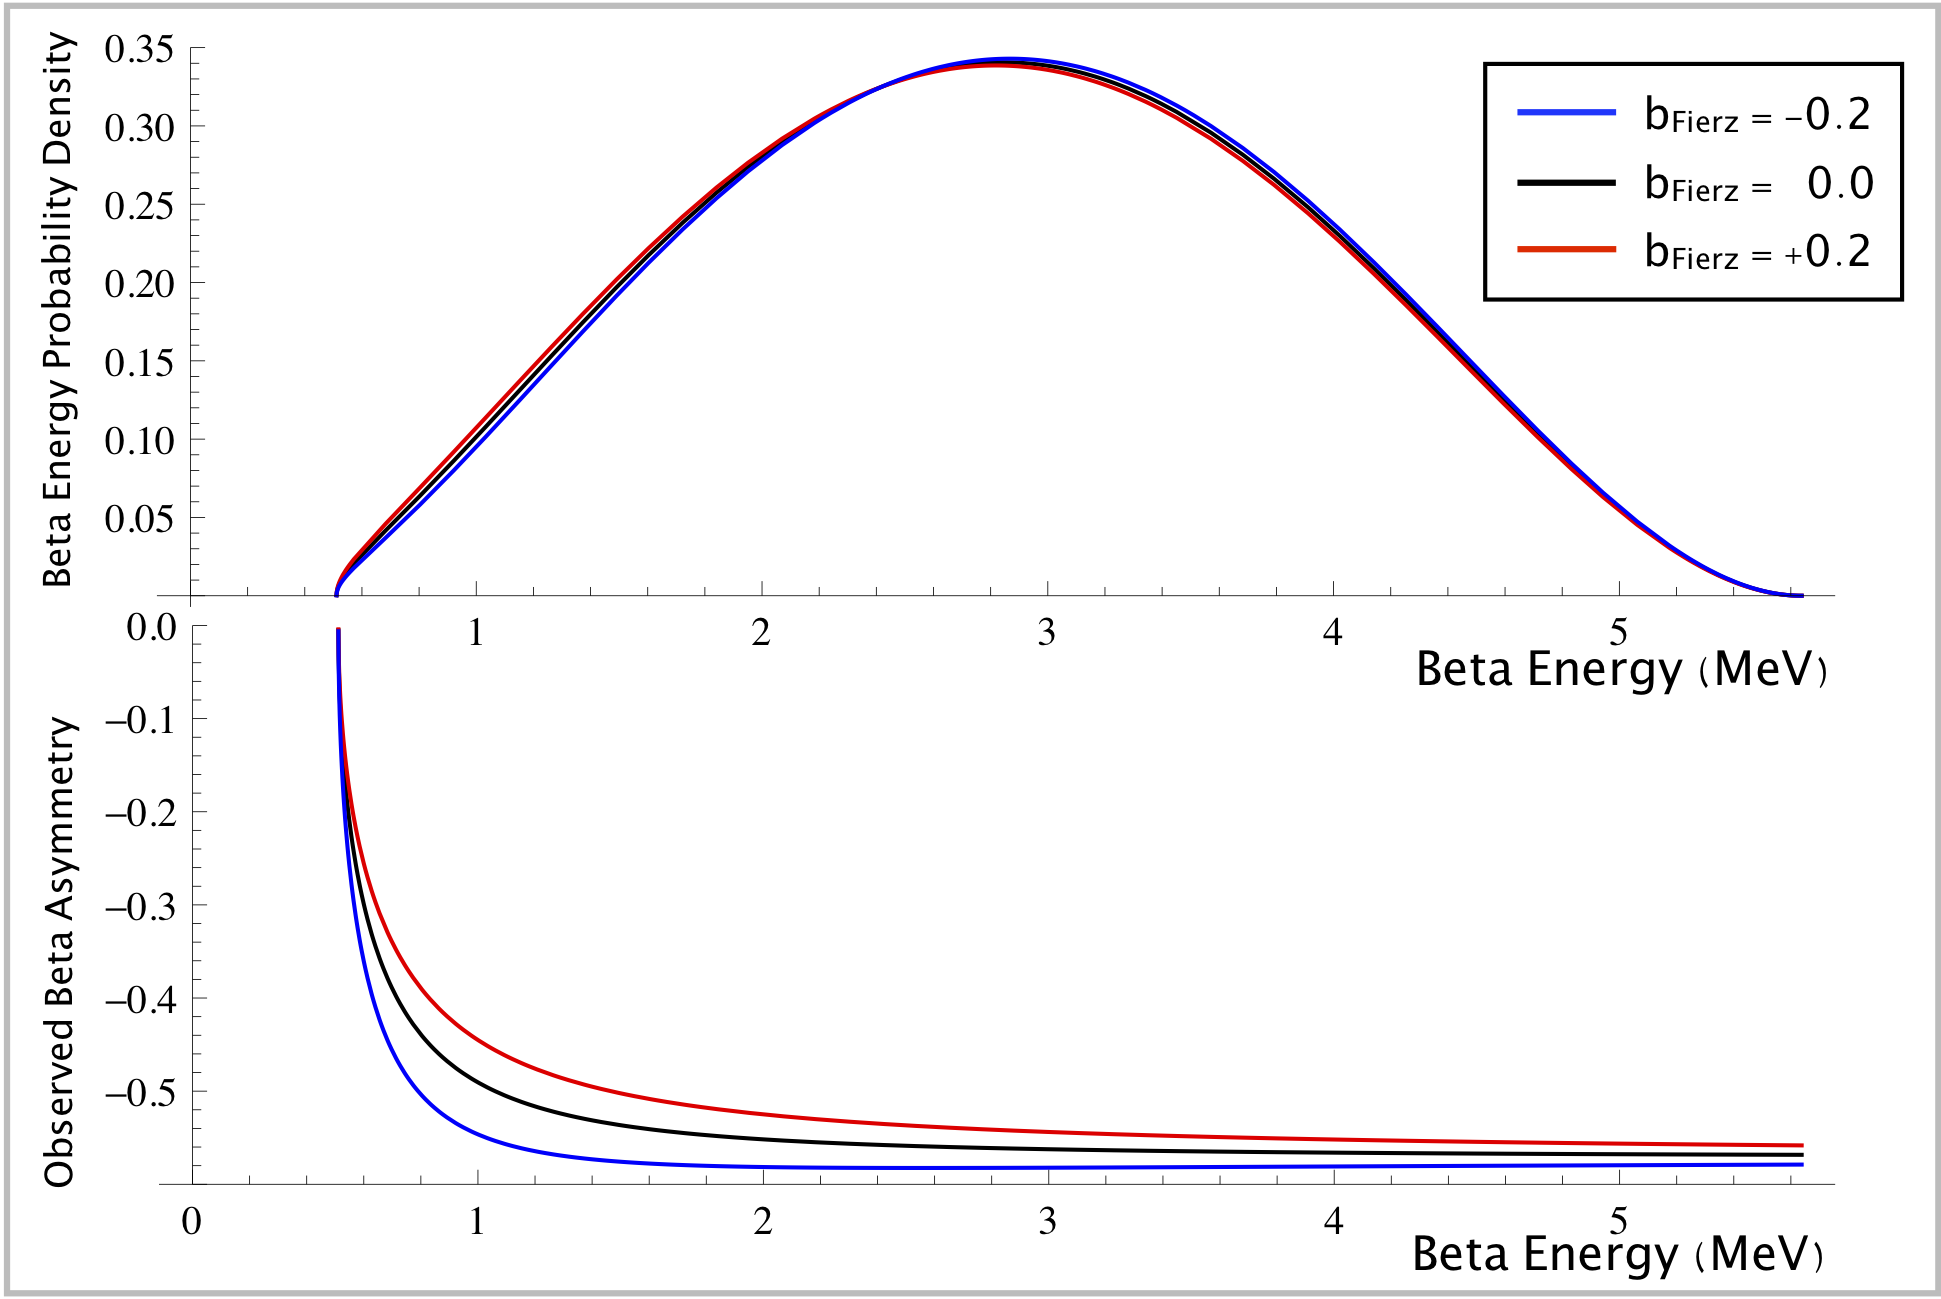
\includegraphics[width=.999\linewidth]
	{Figures/Fierz_Signature.png}
	\caption[Generated Beta Energy Spectrum and Superratio Asymmetry to Measure $\bFierz$]{A generated beta energy spectrum (top), and the superratio asymmetry associated with it (bottom) are constructed to measure a $\bFierz$ signal at the values shown.  The supersum method of Ref.~\cite{UCNA_first_Fierz} is roughly equivalent to constructing the top plot's beta energy spectrum.  Note that the magnitude of these $\bFierz$ values has been made to be unphysically large so that the effect to the top plot can be seen; both scalar and tensor couplings of the size needed to produce this effect have already been ruled out. }	\label{fig:FierzSignature}
\end{figure}

The superratio and superratio asymmetry are discussed in detail within Appendix~\ref{appendix:superratio}.  The discussion includes details on which sort of systematic errors will cancel out entirely, or to leading order, with this treatment -- however it must be noted that for the present project, higher-order corrections are included in all simulations, and the effects are propagated through to the end of the analysis.  Though many systematic effects can be reduced by using the superratio asymmetry, they must still be evaluated.  Therefore, measured values of $\Abeta$ and $\bFierz$ may be directly compared to theoretical predictions.



\note{}
%%%% --- * --- %%%%

\note[done, nolist]{By normalizing Eq.~\ref{equation:integrated_jtw_INTRODUCTION} to have a conventional angular distribution 1 + (term)*$\Abeta$, we can write 
$W(\theta) = 1 + \Abeta/(1+\bFierz \E/\me) cos(\theta) 
\approx 
1 + \Abeta cos(\theta) - \bFierz \E/\me \Abeta cos(\theta) $
for small $\bFierz$.
Our  superratio observable measures directly the coefficient of the $cos(\theta)$ term., and its distortion with energy is multiplied by $\bFierz \Abeta$.
}
\note[jbn]{
The 37K $\Abeta$ is much larger than the neutron's $\Abeta$, so we gain in sensitivity compared to the neutron.
}

\note[jb1]{JB on simple things still missing:
\\
Intro or theory section:
\\...\\
P(cos(theta)) = 1 + bm/E + P  Abeta v/c cos(theta)
\\
where theta is the angle between beta and polarization direction
\\...\\
Higher-order corrections to this equation (citing your appendices and/or
chapters) are included in the simulation,
so you are extracting b and Abeta in this
equation to be compared with theory
\\...\\
\{This is a simple but vital statement-- some people actually extract Abeta(Ebeta$=$0) without recoil-order corrections, which is not the same parameter.\}
\\...\\
The theory prediction for Abeta (citing Fenker PRL) is X.
\\
The theory prediction for bFierz is 0 (maybe you have that already).
}

\note[jb1]{JB on that missing figure that I've now put in:    ``A dependence of Abeta on beta energy is also introduced.
\\
UCNA fits energy spectrum and Abeta[Ebeta] simultaneously now."
}

\note{The point is, the presence of either scalar or tensor interactions will produce a $\bFierz$ term in the decay PDF.  It has other effects on the PDF, but those come in at higher-order in the tiny scalar and tensor couplings.  So, the Fierz term would be by far the biggest thing that changes in the PDF.  The PDF describes the energy and momentum of the outgoing beta w.r.t. a variety of other things.  Notably, we can write an elegant-ish description of beta momentum w.r.t. nuclear polarization direction, and ignore the neutrino completely after integrating over it.  We have a PDF in beta \emph{direction} (w.r.t. polarization), and beta \emph{energy}.  To lowest order (and lowest order is best order) the distribution w.r.t. polarization direction doesn't change, but the distribution w.r.t. energy does change.  Or ... something?  The point is, it makes a change in the beta energy spectrum.  This change is most pronounced at low energies, because the Fierz term is scaled by $(1/\Ebeta)$.  However, the asymmetry is also a function of $\Ebeta$.  A different function of $\Ebeta$.  In fact, it is scaled by $(\pbeta/\Ebeta)$ within the PDF, which is distinctly different than $\bFierz$.  So, one might ask what effect a $\bFierz$ term would produce on a constructed asymmetry spectrum.  ....This explanation has gone way off track.}

\note[done,nolist]{JB:  You need to at some point say that the supersum is the beta energy spectrum.  There are experiments trying to do this method better, but they are very difficult.  UCNA published a combined energy spectrum and Abeta[Ebeta] analysis on the neutron in March 2020~\cite{NeutronbFierz_March2020}.
\\...\\
MJA:  I can't help but also notice the follow-up article from September 2020~\cite{Saul2020}.  Ugh. 
}


















%%%% --- * --- %%%%
\section{Our Decay}
Here, we will focus on the decay,
\bea
^{37}\textrm{K} &\rightarrow& \,^{37}\textrm{\!Ar} + \beta^{+} + \nu_e, 
\label{eq:ourdecay}
\eea
which is extremely well suited to the type of experiment to be the discussed in this thesis.  
%this and other similar experiments -- both because of its suitability 
The parent, $^{37}\textrm{K}$, is an isotope of potassium---an alkali.  Though this fact may initially seem unremarkable, it is their hydrogen-like~\aside[done, nolist]{hydrogen-like does not need quotes} single valence electron which allows alkalis to be readily trapped within a magneto-optical trap, a critical component of our experimental design (see Chapter~\ref{atomicphysics_chapter}).

A potential concern in any experiment concerned with the angular correlations resulting from one particular decay branch is the background from competing decay branches.  As can be seen in Fig.~\ref{fig:nuclearleveldiagram}, the decay of $^{37}\textrm{K}$ is dominated by a single branch which contributes nearly $98\%$ of $^{37}\textrm{K}$ decay events, and the remaining events nearly all arise from a single branch contributing around $2\%$ of the decay events.  The other branches combined account for only around $0.04\%$ of decays.  Taken all together, this means that the background events which must be accounted for are both infrequent and well understood.

\begin{figure}[h!t!b!]
	\centering
	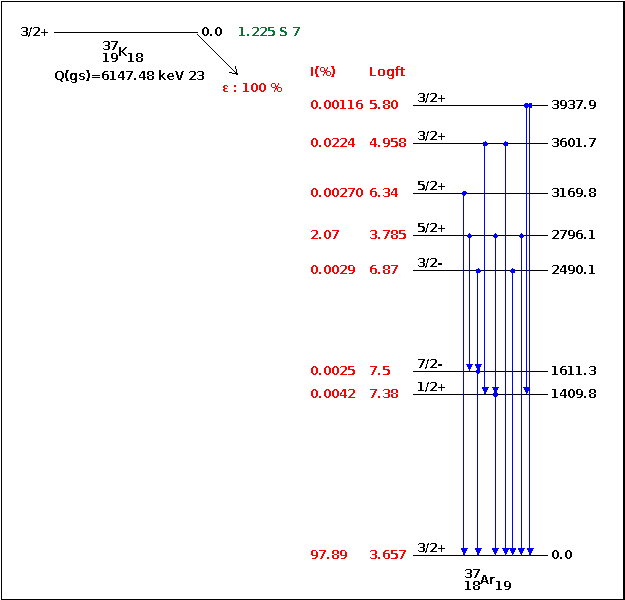
\includegraphics[width=.999\linewidth]{Figures/decayscheme_nndc.png}
	\caption[Decay Scheme for $^{37}$K]{A Decay Scheme for $^{37}$K, generated with the NuDat3 database toolset.  The $I(\%)$ column indicates the fraction of total decays which proceed to each level, and `Logft' gives a measure of the absolute decay rate\cite{krane}.  The column immediately to the right  of Logft indicates nuclear spin and parity, and the far right column is the energy relative to the ground state, in keV\cite{nucleardata2012}\cite{shidling2014}\cite{ozmetin2020}. 
	}	
	\label{fig:nuclearleveldiagram}
\end{figure}
%\FloatBarrier

\note{Re: Fig.~\ref{fig:nuclearleveldiagram}:  the picture needs needs:  title, labels on $I^\pi$ columns, label "energy" on the RH column (which kind of energy?  It's the "level energy".  
}
\note[done, nolist]{JB says Re: Fig.~\ref{fig:nuclearleveldiagram}: 
\\..\\
The caption should include that [...] log\_10(fT) [is] a measure of the absolute decay rate (ref. Krane e.g.) \cite{krane}.
the [...] column [that] has $I^\pi$ where I is spin and $\pi$ is parity [should get a label]. This should not only include Dan's thesis for a reference, but the most recent paper with the branches-- it should work to reference P.D. Shidling
et al. Phys Rev C 98 015502 (2018) \cite{shidling2014} which re-did the half-life and summarized the fT value extraction. I see no publication of your branching ratio work, so I referenced Ozmetin's DNP talk in an earlier note. \cite{ozmetin2020}
}


As in any decay, the angular correlations between the emerging daughter particles provide a rich source of information about the type of interaction that produced the decay.  
This particular decay involves a set of isobaric mirror nuclei, meaning that the nuclear wavefunctions of the parent and daughter are identical up to their isospin quantum number and corresponding electrical charge.  Because the two wavefunctions are so similar, effects to the decay from nuclear structure corrections are well understood and can be kept to a minimum, making it possible to place especially strong constraints on the size of the theoretical uncertainties associated with the decay.
%Because the higher-order standard model corrections to this decay process are well understood, it is an ideal candidate for for improving constraints on interactions beyond the standard model.  

\note[done, nolist]{no one will let you publish air quotes, ever. Have mercy on your committee, take them all out.  Use the opportunity to make sure you've defined them.
\\...\\
Here, just say isobaric mirror nuclei. You define it right there in text. It's fine to use textbook terms as long as you define them immediately.} 
\note[bluetodo]{Is it definitely true that the nuclear structure corrections are *smaller*?  Or is it just that they're better understood?}

\note{Also, 37K is a really nice isotope for this, because 
%98\% + 2\%, 
%also because it's a mirror decay, 
%also because it's an alkali.  Also-
%also, 
its big $\Abeta$ value means we have a big thing to multiply any $\bFierz$ value there might be when we construct the superratio asymmetry to eliminate systematics.}

%\missingfigure{This thing is going to need a nuclear level diagram for 37K.  Also, 37K is a really nice isotope for this, because 98\% + 2\%, also because it's a mirror decay, also because it's an alkali.  Also-also, its big $\Abeta$ value means we have a big thing to multiply any $\bFierz$ value there might be when we construct the superratio asymmetry to eliminate systematics.}




%%%% --- * --- %%%%	
\section{The Shake-off Electron Spectrum}
\label{section:soe_intro}
Although the beta decay process is primarily concerned with the emission of beta particles (electrons or positrons) from a Weak interaction that occurs within the nucleus, it is common for one or more \emph{orbital} electrons to also be lost in the process.  Although beta particles are emitted over a continuous energy spectrum, they commonly carry several MeV of kinetic energy.  By contrast, an atomic electron that becomes unbound in this process is likely to only carry a few eV of kinetic energy.  These are referred to as \acp{SOE}, since they are in some sense shaken off.

We will amend Eq.~\ref{eq:ourdecay} to reflect the presence of $N$ such \ac{SOE}s within each decay event, as
\bea
^{37}\textrm{K} &\rightarrow& \,^{37}\textrm{\!Ar}^{(N-1)+} + \beta^{+} + \nu_e + N \, e_{\textrm{SO}}, 
\label{eq:ourdecay_withsoe}
\eea
%\aside{Do I want to re-assign N somehow so the notation works better?}
where it is clear that, since the parent $^{37}\textrm{K}$ atom was electrically neutral before its decay by $\beta^+$ emission, the daughter $^{37}\textrm{\!Ar}$ will initially have an extra
%~\aside[jbn]{'extra' -> extra. You're not breaking charge conservation here, you don't need to define the word.} 
orbital electron (and therefore a negative net charge) if no electrons are shaken off.  We also note that it is common for multiple SOEs to be created in a given decay event.  

A further consideration is that the outer electron in an $^{37}\textrm{\!Ar}^{-}$ ion is not bound\cite{ArgonMinusIons}, and in an electric field such as is present within our experimental chamber, this outer electron is removed immediately to be accelerated through the field, leaving behind a neutral $^{37}\textrm{\!Ar}$ atom.  Although this is in principle a different physical loss mechanism, we will refer to unbound electrons resulting from either process as SOEs.  

It is useful to consider the energy spectrum of these shake-off electrons.  The most straightforward component of the SOE energy spectrum arises from the electrons that are lost immediately following decay, and we take these to initially have 0eV in kinetic energy.  

For the shake-off electrons arising from the Weak process itself, the initial energy spectra for SOEs originating in a particular orbital shell can be estimated according to the procedure outlined by Levinger, who credits Feynman for the suggestion~\cite{Levinger}.
~\note[done, nolist]{JB:  \\
$\rightarrow$``by Levinger, who credits Feynman for the suggestion~\cite{Levinger}.''
\\...\\
(Since this is a true story that is not embellished by Feynman in someone else's joke book, but is in a footnote in the Physical Review,  I like to mention it.)
}  \noindent
The strategy is to assume that the sudden approximation holds, and simply calculate the overlap in electron wavefunctions between the initial and final states, where the final state may be either an outgoing electron or one bound within the atom.  Analytic expressions can be obtained if the atom is treated as being hydrogenic -- an excellent approximation here, as $^{37}\textrm{K}$ is an alkali.  

Unfortunately, this treatment cannot determine the fractional contribution of each orbital to the total, nor can it determine the \emph{number} of electrons likely to be removed in a single decay event.  The implications of the SOE energy spectrum to the present experiment are discussed further in Section~\ref{sec:tof_bg}.

\note[bluetodo]{In the end, we used $(0.09)*(\textrm{0eV}) + (0.91)*(0.85*(\textrm{4S}) + 0.15*(\textrm{3P}))$.  But I say that in the other section.  Also, John used Eq.20 for the 4S, and Eq.24 for the 3P.}
\note{Comment on how well this matches our data?  Somehow?}

%\note{Should I talk about the distribution of how many SOEs come off in a decay?  I have measurements of the recoil charge distribution, which is related but not really the same thing.  From a theoretical POV, I don't know how many get shaken off.  Thankfully, it doesn't matter very much in the end.}

%%%%%\begin{figure}[h!!t]
%%%%%	\centering
%%%%%	\includegraphics[width=.999\linewidth]
%%%%%	{Figures/Levinger_SOETOF_prelim.pdf}
%%%%%	\note[clean]{Clean up SOE TOF pic in intro.  It doesn't show what I need!}
\note{A picture of the SOE spectrum for the intro was here.  It's gone now, but it's important that we remember!  pretty sure I reference it from somewhere else...}
%%%%%	\note{Maybe just kill this picture?  At least reference it in the text somewhere.}
%%%%%	\caption[Levinger TOF]{Shake-off electron TOF (w.r.t. beta TOA) spectrum, showing how the spectrum is different if one includes different sets of initial electrons to be shaken off.  I forget why some of them have 0 eV.  Maybe those are the ones from the $\isotope[37]{Ar}^+$. ... Levinger TOF spectra for some different sets of SOE initial orbitals before shake-off.  (At least that's what it's supposed to be, after I fix the picture).  It's reconstructed event-by-event with beta times-of-flight that would pass some basic `good event' cuts.  Anyway, it turns out, it doesn't much matter what orbitals you lose SOEs from.  That's nice.  In the end, I used 85+15.  \comment{(Need to re-plot this.)} }	
%%%%%	\label{fig:levinger_TOF}
%%%%%\end{figure}



